

\begin{frame}{Watset: synset induction}
	\textbf{ACL'17}~\cite{ustalov-panchenko-biemann:2017:Long}
	
	
	%\block{Sample Synsets Induced by the \watset{[MCL, MCL]} Method for English}{
\vspace{1em}
Examples of extracted synsets:
\vspace{1em}
\centering
\begin{tabular}{c|p{9cm}}
\textbf{Size} & \textbf{Synset}\\\hline
2 & \{\textit{decimal point}, \textit{dot}\}\\
3 & \{\textit{gullet}, \textit{throat}, \textit{food pipe}\}\\
4 & \{\textit{microwave meal}, \textit{ready meal}, \textit{TV dinner}, \textit{frozen dinner}\}\\
5 & \{\textit{objective case}, \textit{accusative case}, \textit{oblique case}, \textit{object case}, \textit{accusative}\}\\
6 & \{\textit{radio theater}, \textit{dramatized audiobook}, \textit{audio theater}, \textit{radio play}, \textit{radio drama}, \textit{audio play}\}\\
\end{tabular}


	
	
\end{frame}


\begin{frame}{Synset induction}
	
	
Outline of the 'Watset' method:

\vspace{2em}

\centering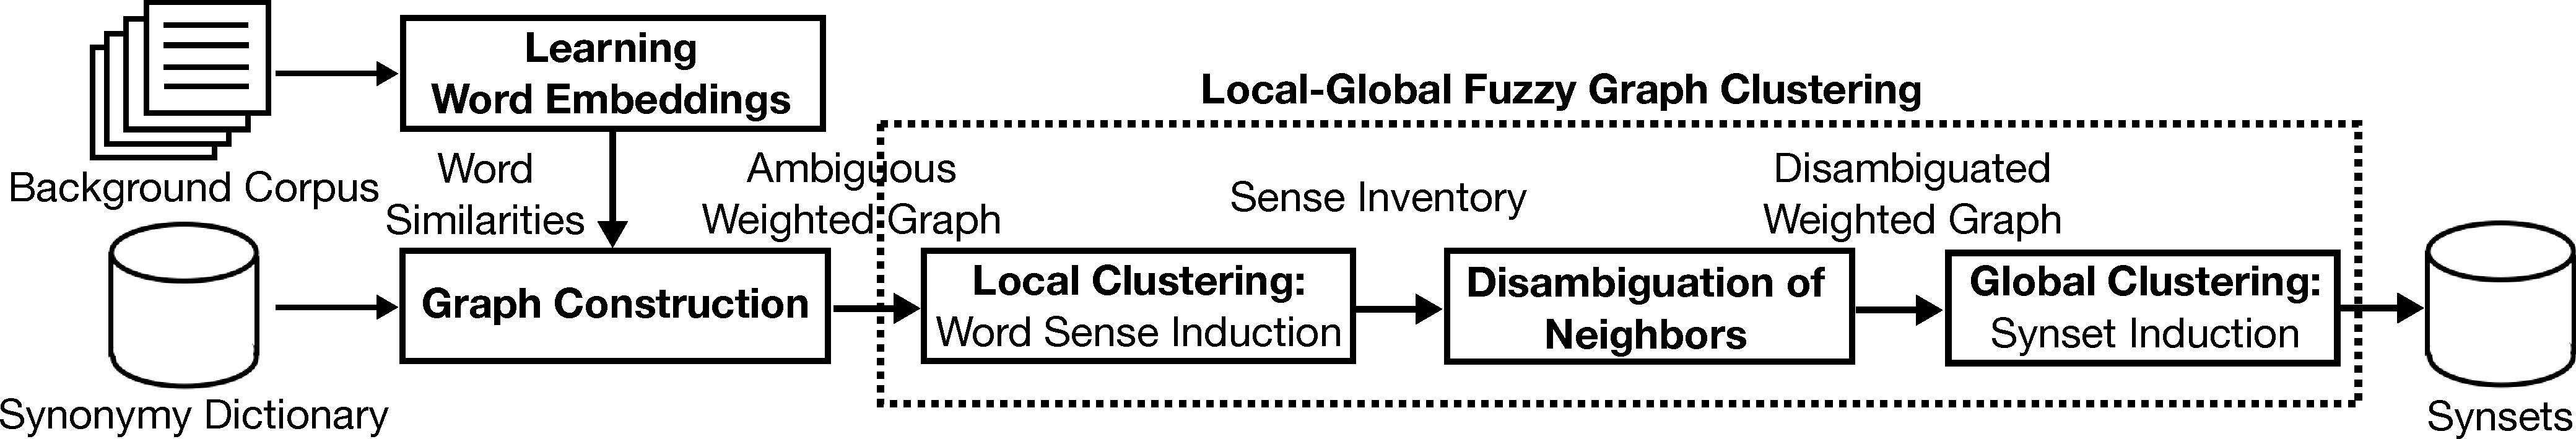
\includegraphics[width=1.05\textwidth]{outline}
	
\end{frame}


\begin{frame}{Synset induction}
\centering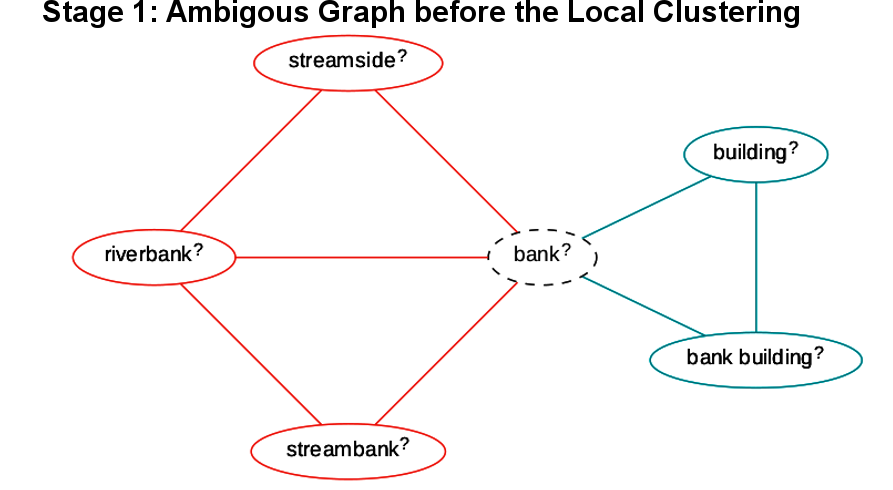
\includegraphics[width=1\textwidth]{stages1}	
\end{frame}



\begin{frame}{Synset induction}
\centering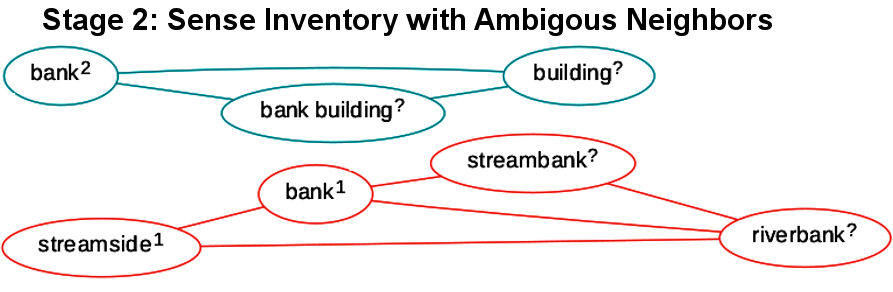
\includegraphics[width=1\textwidth]{stages2}	
\end{frame}



\begin{frame}{Synset induction}
\centering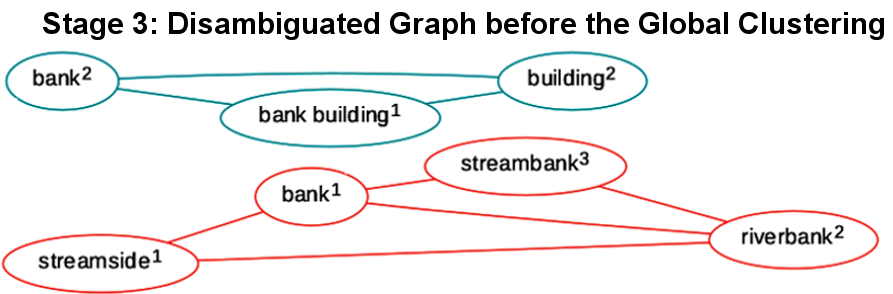
\includegraphics[width=1\textwidth]{stages3}	
\end{frame}


\begin{frame}{Synset induction}

  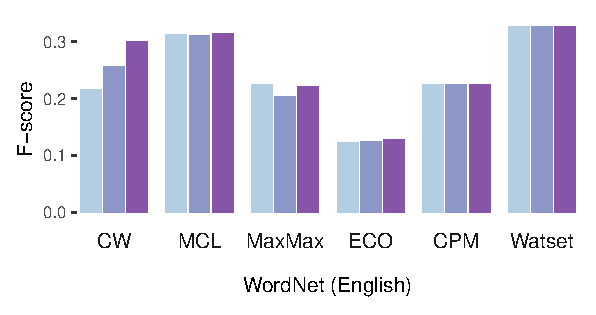
\includegraphics[width=0.49\textwidth]{edges-en-wordnet}  
  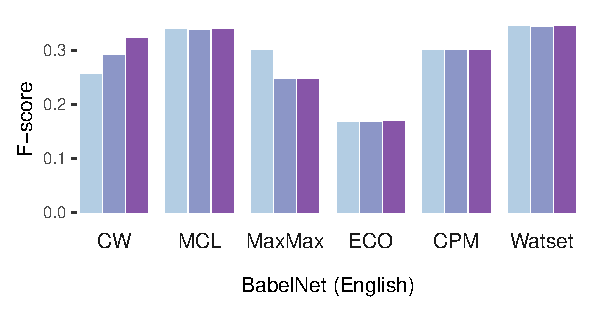
\includegraphics[width=0.49\textwidth]{edges-en-babelnet}

  \pause    
  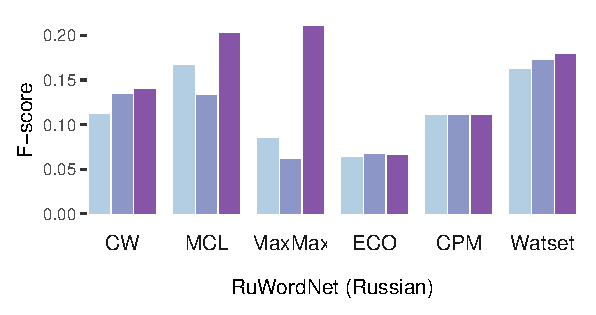
\includegraphics[width=0.49\textwidth]{edges-ru-rwn}     
  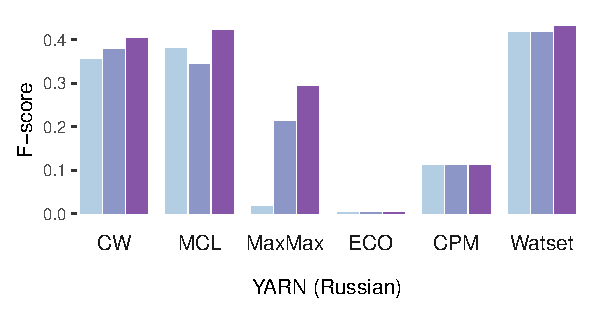
\includegraphics[width=0.49\textwidth]{edges-ru-yarn}     
	
\end{frame}



\begin{frame}{Induction of  semantic classes}
	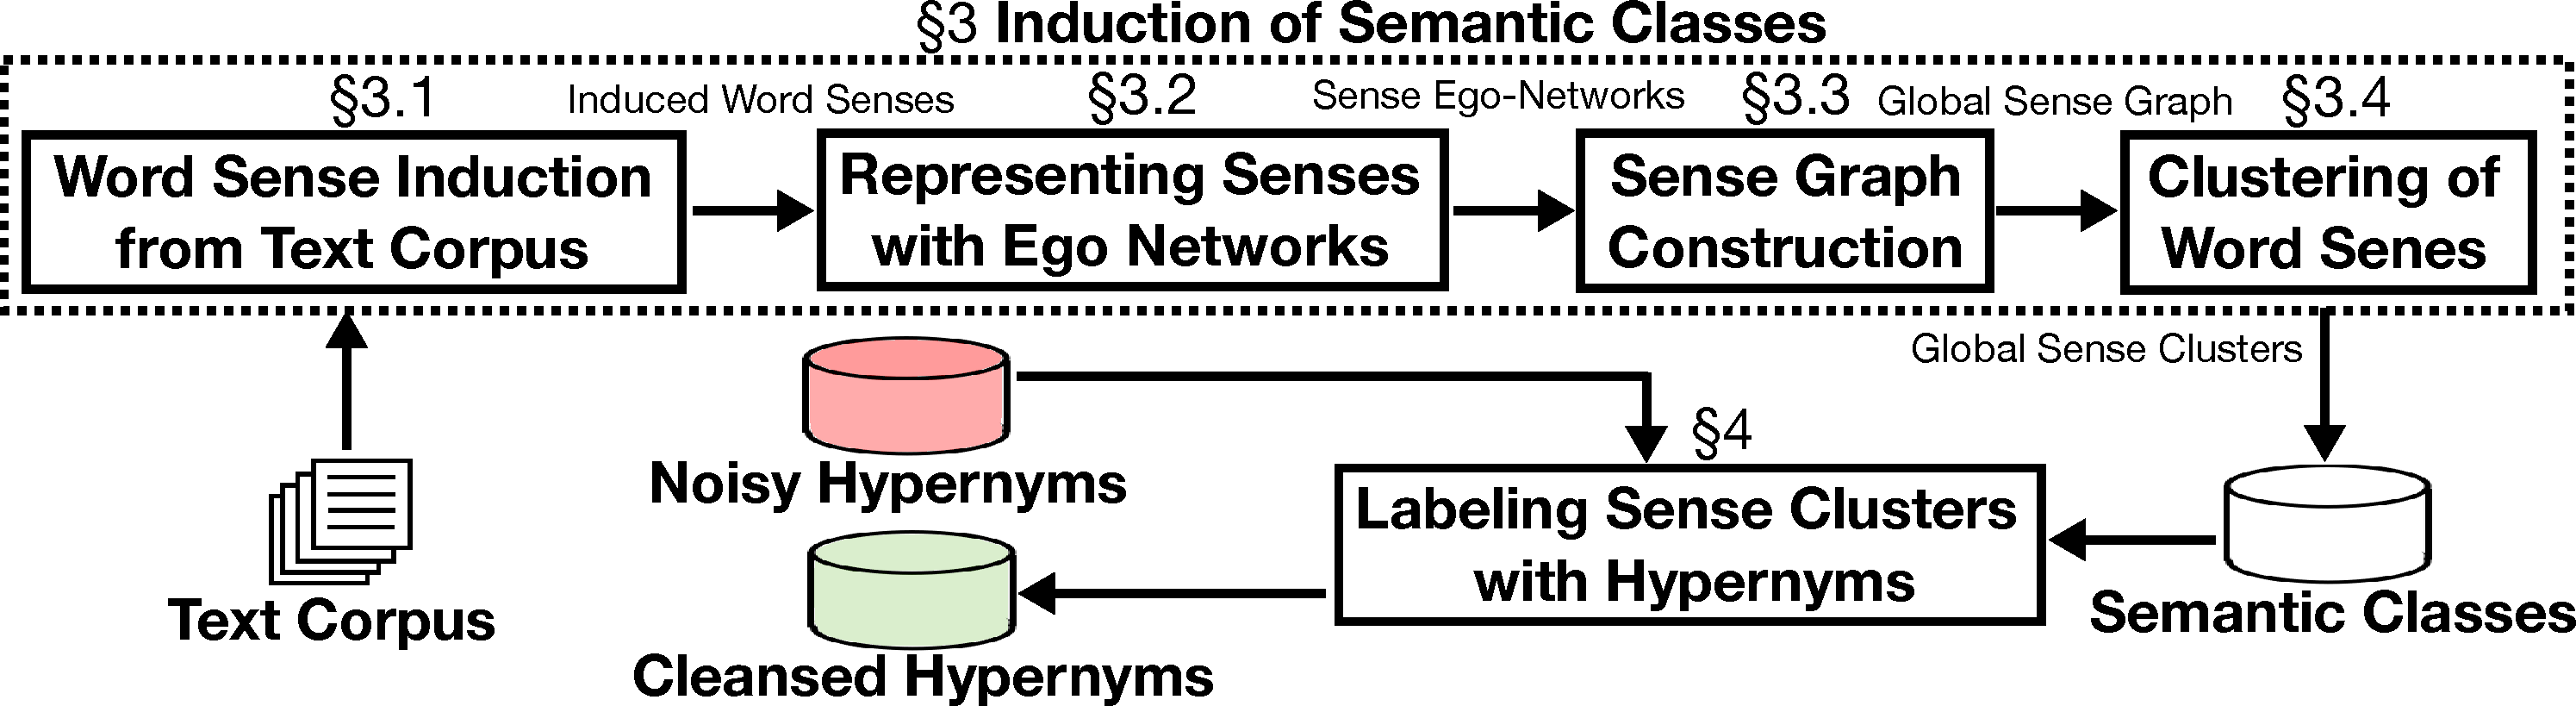
\includegraphics[width=1.0\textwidth]{semantic-classes-outline}
\end{frame}


\begin{frame}{Induction of  semantic classes}

Examples of semantic classes:


\begin{table}[ht]
\centering
\scriptsize
\begin{tabular}{l|p{6cm}|p{3.5cm}} 

\bf ID &  \bf Sense Cluster & \bf Hypernyms \\ \hline
& &  \\
1 & peach\#1, banana\#1, pineapple\#0, berry\#0, blackberry\#0, grapefruit\#0, strawberry\#0, blueberry\#0, fruit\#0, grape\#0, melon\#0, orange\#0, pear\#0, plum\#0, raspberry\#0, watermelon\#0, apple\#0, apricot\#0, ...  &  vegetable\#0, fruit\#0, crop\#0, ingredient\#0, food\#0, $\cdot$ \\ & &  \\ \hline
& &  \\
2  & C\#4, Basic\#2, Haskell\#5, Flash\#1, Java\#1, Pascal\#0, Ruby\#6, PHP\#0, Ada\#1, Oracle\#3, Python\#3, Apache\#3, Visual Basic\#1, ASP\#2, Delphi\#2, SQL Server\#0, CSS\#0, AJAX\#0, the Java\#0, ... & programming language\#3, technology\#0, language\#0, format\#2, app\#0 
\end{tabular}
\end{table}

	
\end{frame}



\begin{frame}{Induction of sense semantic classes}

Filtering noisy hypernyms with semantic classes \textbf{LREC'18}~\cite{panchenko:2018:SemanticClasses}: 

	\centering 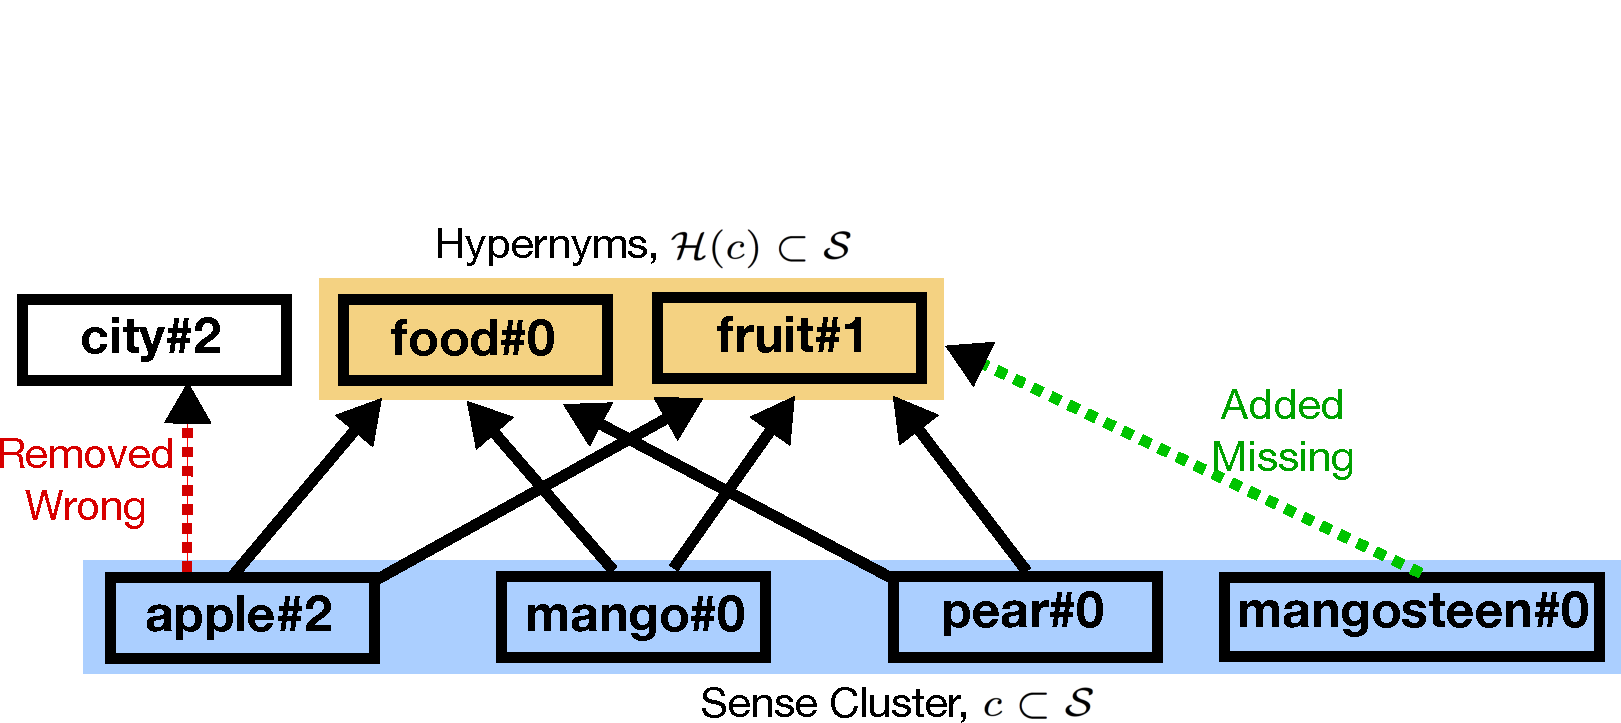
\includegraphics[width=1.0\textwidth]{coset}
	
\end{frame}


\begin{frame}{Induction of sense semantic classes}

Filtering of a noisy hypernymy database with semantic classes.  \textbf{LREC'18}~\cite{panchenko:2018:SemanticClasses}

\begin{table}
\scriptsize
\centering
\resizebox{1.0\linewidth}{!}{
\begin{tabular}{l|c|c|c}
 & \textbf{Precision} & \textbf{Recall} & \textbf{F-score} \\ \hline
Original Hypernyms  (Seitner et al., 2016) & $0.475$ & $0.546$ & $0.508$ \\
Semantic Classes (coarse-grained) & $\mathbf{0.541}$ & $\mathbf{0.679}$ & $\mathbf{0.602}$ \\
\end{tabular}
}
\end{table}
	
\end{frame}




